\documentclass[twoside]{book}

% Packages required by doxygen
\usepackage{fixltx2e}
\usepackage{calc}
\usepackage{doxygen}
\usepackage[export]{adjustbox} % also loads graphicx
\usepackage{graphicx}
\usepackage[utf8]{inputenc}
\usepackage{makeidx}
\usepackage{multicol}
\usepackage{multirow}
\PassOptionsToPackage{warn}{textcomp}
\usepackage{textcomp}
\usepackage[nointegrals]{wasysym}
\usepackage[table]{xcolor}

% Font selection
\usepackage[T1]{fontenc}
\usepackage[scaled=.90]{helvet}
\usepackage{courier}
\usepackage{amssymb}
\usepackage{sectsty}
\renewcommand{\familydefault}{\sfdefault}
\allsectionsfont{%
  \fontseries{bc}\selectfont%
  \color{darkgray}%
}
\renewcommand{\DoxyLabelFont}{%
  \fontseries{bc}\selectfont%
  \color{darkgray}%
}
\newcommand{\+}{\discretionary{\mbox{\scriptsize$\hookleftarrow$}}{}{}}

% Page & text layout
\usepackage{geometry}
\geometry{%
  a4paper,%
  top=2.5cm,%
  bottom=2.5cm,%
  left=2.5cm,%
  right=2.5cm%
}
\tolerance=750
\hfuzz=15pt
\hbadness=750
\setlength{\emergencystretch}{15pt}
\setlength{\parindent}{0cm}
\setlength{\parskip}{3ex plus 2ex minus 2ex}
\makeatletter
\renewcommand{\paragraph}{%
  \@startsection{paragraph}{4}{0ex}{-1.0ex}{1.0ex}{%
    \normalfont\normalsize\bfseries\SS@parafont%
  }%
}
\renewcommand{\subparagraph}{%
  \@startsection{subparagraph}{5}{0ex}{-1.0ex}{1.0ex}{%
    \normalfont\normalsize\bfseries\SS@subparafont%
  }%
}
\makeatother

% Headers & footers
\usepackage{fancyhdr}
\pagestyle{fancyplain}
\fancyhead[LE]{\fancyplain{}{\bfseries\thepage}}
\fancyhead[CE]{\fancyplain{}{}}
\fancyhead[RE]{\fancyplain{}{\bfseries\leftmark}}
\fancyhead[LO]{\fancyplain{}{\bfseries\rightmark}}
\fancyhead[CO]{\fancyplain{}{}}
\fancyhead[RO]{\fancyplain{}{\bfseries\thepage}}
\fancyfoot[LE]{\fancyplain{}{}}
\fancyfoot[CE]{\fancyplain{}{}}
\fancyfoot[RE]{\fancyplain{}{\bfseries\scriptsize Generated by Doxygen }}
\fancyfoot[LO]{\fancyplain{}{\bfseries\scriptsize Generated by Doxygen }}
\fancyfoot[CO]{\fancyplain{}{}}
\fancyfoot[RO]{\fancyplain{}{}}
\renewcommand{\footrulewidth}{0.4pt}
\renewcommand{\chaptermark}[1]{%
  \markboth{#1}{}%
}
\renewcommand{\sectionmark}[1]{%
  \markright{\thesection\ #1}%
}

% Indices & bibliography
\usepackage{natbib}
\usepackage[titles]{tocloft}
\setcounter{tocdepth}{3}
\setcounter{secnumdepth}{5}
\makeindex

% Hyperlinks (required, but should be loaded last)
\usepackage{ifpdf}
\ifpdf
  \usepackage[pdftex,pagebackref=true]{hyperref}
\else
  \usepackage[ps2pdf,pagebackref=true]{hyperref}
\fi
\hypersetup{%
  colorlinks=true,%
  linkcolor=blue,%
  citecolor=blue,%
  unicode%
}

% Custom commands
\newcommand{\clearemptydoublepage}{%
  \newpage{\pagestyle{empty}\cleardoublepage}%
}

\usepackage{caption}
\captionsetup{labelsep=space,justification=centering,font={bf},singlelinecheck=off,skip=4pt,position=top}

%===== C O N T E N T S =====

\begin{document}

% Titlepage & ToC
\hypersetup{pageanchor=false,
             bookmarksnumbered=true,
             pdfencoding=unicode
            }
\pagenumbering{alph}
\begin{titlepage}
\vspace*{7cm}
\begin{center}%
{\Large iperf G\+UI }\\
\vspace*{1cm}
{\large Generated by Doxygen 1.8.12}\\
\end{center}
\end{titlepage}
\clearemptydoublepage
\pagenumbering{roman}
\tableofcontents
\clearemptydoublepage
\pagenumbering{arabic}
\hypersetup{pageanchor=true}

%--- Begin generated contents ---
\chapter{Hierarchical Index}
\section{Class Hierarchy}
This inheritance list is sorted roughly, but not completely, alphabetically\+:\begin{DoxyCompactList}
\item Q\+Widget\begin{DoxyCompactList}
\item \contentsline{section}{Client}{\pageref{class_client}}{}
\item \contentsline{section}{Num\+Pad}{\pageref{class_num_pad}}{}
\item \contentsline{section}{Server}{\pageref{class_server}}{}
\item \contentsline{section}{Traffic\+Light}{\pageref{class_traffic_light}}{}
\item \contentsline{section}{Welcome\+Screen}{\pageref{class_welcome_screen}}{}
\end{DoxyCompactList}
\end{DoxyCompactList}

\chapter{Class Index}
\section{Auflistung der Klassen}
Hier folgt die Aufzählung aller Klassen, Strukturen, Varianten und Schnittstellen mit einer Kurzbeschreibung\+:\begin{DoxyCompactList}
\item\contentsline{section}{\hyperlink{class_client}{Client} \\*Die Client-\/\+Klasse }{\pageref{class_client}}{}
\item\contentsline{section}{\hyperlink{class_iperf_interface}{Iperf\+Interface} \\*Die Iperf\+Interface-\/\+Klasse }{\pageref{class_iperf_interface}}{}
\item\contentsline{section}{\hyperlink{class_num_pad}{Num\+Pad} \\*Die Num\+Pad-\/\+Klasse }{\pageref{class_num_pad}}{}
\item\contentsline{section}{\hyperlink{class_server}{Server} \\*Die Server-\/\+Klasse }{\pageref{class_server}}{}
\item\contentsline{section}{\hyperlink{class_traffic_light}{Traffic\+Light} \\*Die Traffic\+Light-\/\+Klasse }{\pageref{class_traffic_light}}{}
\item\contentsline{section}{\hyperlink{class_welcome_screen}{Welcome\+Screen} \\*Die Welcome\+Screen-\/\+Klasse }{\pageref{class_welcome_screen}}{}
\end{DoxyCompactList}

\chapter{File Index}
\section{File List}
Here is a list of all documented files with brief descriptions\+:\begin{DoxyCompactList}
\item\contentsline{section}{src/\hyperlink{client_8h}{client.\+h} \\*A brief description about this header file }{\pageref{client_8h}}{}
\item\contentsline{section}{src/\hyperlink{main_8cpp}{main.\+cpp} \\*The main file of this project }{\pageref{main_8cpp}}{}
\item\contentsline{section}{src/{\bfseries numpad.\+h} }{\pageref{numpad_8h}}{}
\item\contentsline{section}{src/{\bfseries server.\+h} }{\pageref{server_8h}}{}
\item\contentsline{section}{src/{\bfseries trafficlight.\+h} }{\pageref{trafficlight_8h}}{}
\item\contentsline{section}{src/{\bfseries welcomescreen.\+h} }{\pageref{welcomescreen_8h}}{}
\end{DoxyCompactList}

\chapter{Class Documentation}
\hypertarget{class_client}{}\section{Client Klassenreferenz}
\label{class_client}\index{Client@{Client}}


Die Client-\/\+Klasse.  




{\ttfamily \#include $<$client.\+h$>$}

Klassendiagramm für Client\+:\begin{figure}[H]
\begin{center}
\leavevmode
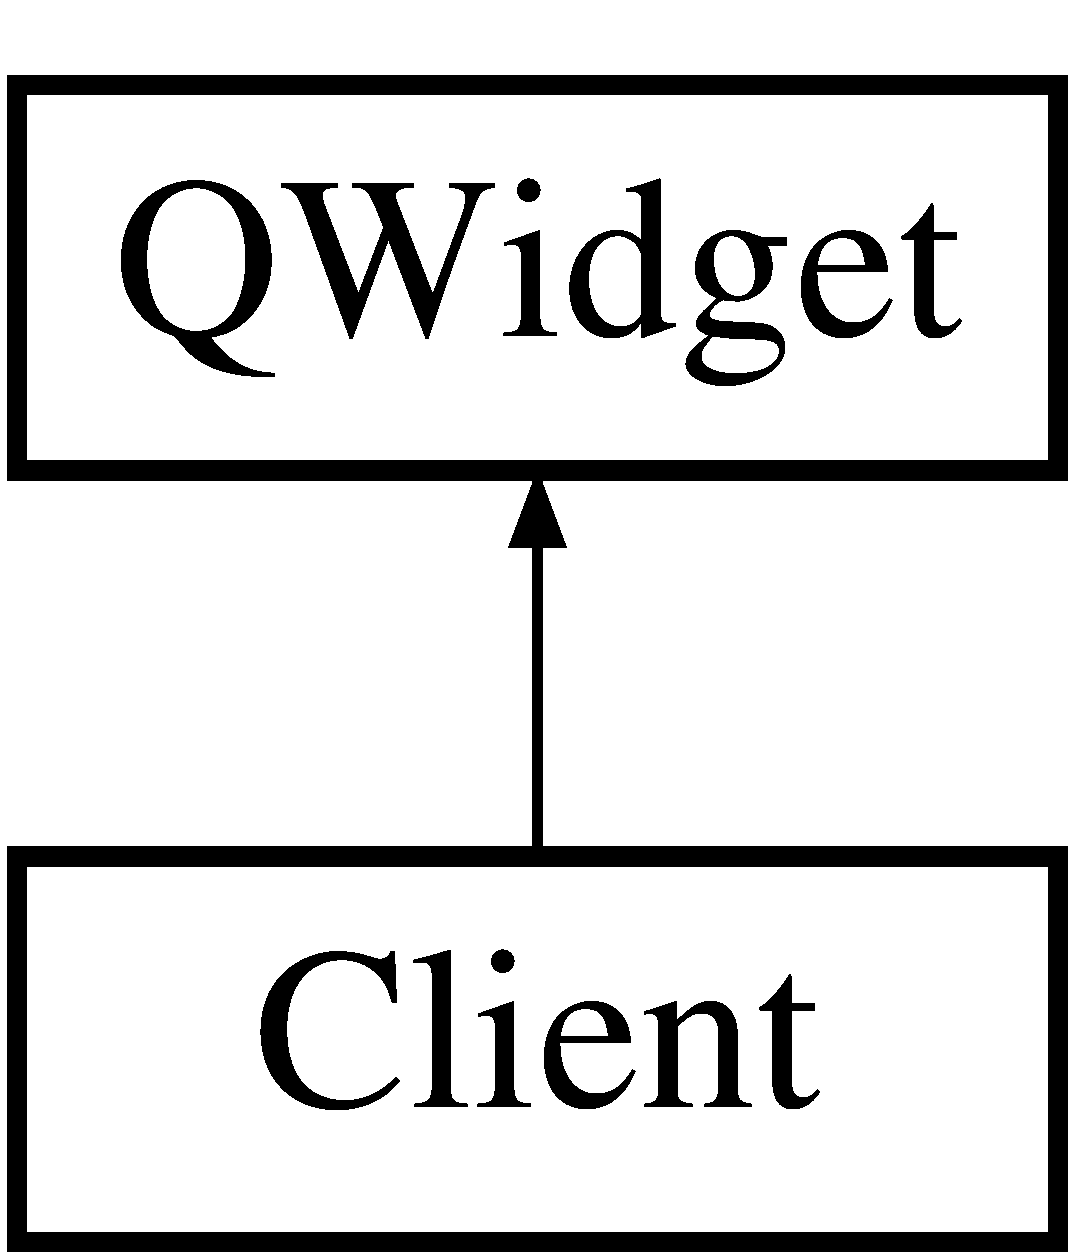
\includegraphics[height=2.000000cm]{class_client}
\end{center}
\end{figure}
\subsection*{Öffentliche Slots}
\begin{DoxyCompactItemize}
\item 
\hypertarget{class_client_a5f96334ebe2c8a22f6448cff80d027a5}{}\label{class_client_a5f96334ebe2c8a22f6448cff80d027a5} 
void \hyperlink{class_client_a5f96334ebe2c8a22f6448cff80d027a5}{on\+Exit\+Button\+Clicked} ()
\begin{DoxyCompactList}\small\item\em Beim Klicken des Schliessen-\/\+Button aufgerufene Handler-\/\+Methode. \end{DoxyCompactList}\item 
\hypertarget{class_client_aa56b217ce77d6e41f76474ed92378798}{}\label{class_client_aa56b217ce77d6e41f76474ed92378798} 
void \hyperlink{class_client_aa56b217ce77d6e41f76474ed92378798}{on\+Start\+Button\+Clicked} ()
\begin{DoxyCompactList}\small\item\em Beim Klicken des Starten-\/\+Button aufgerufene Handler-\/\+Methode. \end{DoxyCompactList}\item 
\hypertarget{class_client_a548c8d8b2eb95c3ecbec190495940b99}{}\label{class_client_a548c8d8b2eb95c3ecbec190495940b99} 
void \hyperlink{class_client_a548c8d8b2eb95c3ecbec190495940b99}{on\+Keyboard\+Clicked} ()
\begin{DoxyCompactList}\small\item\em Beim Klicken des Keyboard-\/\+Button aufgerufene Handler-\/\+Methode. \end{DoxyCompactList}\item 
\hypertarget{class_client_a8dbb1b513ea96c6016e97cb03d4e6b0d}{}\label{class_client_a8dbb1b513ea96c6016e97cb03d4e6b0d} 
void \hyperlink{class_client_a8dbb1b513ea96c6016e97cb03d4e6b0d}{on\+Runtime\+Changed} (int)
\begin{DoxyCompactList}\small\item\em Beim Bewegen oder Anklicken des Slider \char`\"{}\+Laufzeit\char`\"{} aufgerufene Handler-\/\+Methode. \end{DoxyCompactList}\item 
\hypertarget{class_client_afe033bbce94884369c9b488485f879ad}{}\label{class_client_afe033bbce94884369c9b488485f879ad} 
void \hyperlink{class_client_afe033bbce94884369c9b488485f879ad}{on\+Bandwidth\+Changed} (int)
\begin{DoxyCompactList}\small\item\em Beim Bewegen oder Anklicken des Slider \char`\"{}\+Bandbreite\char`\"{} aufgerufene Handler-\/\+Methode. \end{DoxyCompactList}\item 
\hypertarget{class_client_a01f6d4ddcb338116dc4a4ba320f47456}{}\label{class_client_a01f6d4ddcb338116dc4a4ba320f47456} 
void \hyperlink{class_client_a01f6d4ddcb338116dc4a4ba320f47456}{on\+Client\+Has\+Finished} ()
\begin{DoxyCompactList}\small\item\em Wird aufgerufen sobald der \hyperlink{class_client}{Client} keine Pakete mehr sendet, also beendet ist. \end{DoxyCompactList}\item 
void \hyperlink{class_client_a9699e2db43beff88b4694208c54c1b7f}{set\+IP} (Q\+String s)
\begin{DoxyCompactList}\small\item\em Setzt die I\+P-\/\+Adresse. \end{DoxyCompactList}\item 
Q\+String \hyperlink{class_client_a91bf1f59731649499365d8b18e6aee62}{get\+IP} ()
\begin{DoxyCompactList}\small\item\em Gibt die I\+P-\/\+Adresse zurück. \end{DoxyCompactList}\end{DoxyCompactItemize}
\subsection*{Öffentliche Methoden}
\begin{DoxyCompactItemize}
\item 
\hyperlink{class_client_ab9cb979d7fb7dd0bd3bf645279a6ffb5}{Client} (Q\+Widget $\ast$parent=0)
\begin{DoxyCompactList}\small\item\em \hyperlink{class_client}{Client} Konstruktor. \end{DoxyCompactList}\end{DoxyCompactItemize}


\subsection{Ausführliche Beschreibung}
Die Client-\/\+Klasse. 

\subsection{Beschreibung der Konstruktoren und Destruktoren}
\hypertarget{class_client_ab9cb979d7fb7dd0bd3bf645279a6ffb5}{}\label{class_client_ab9cb979d7fb7dd0bd3bf645279a6ffb5} 
\index{Client@{Client}!Client@{Client}}
\index{Client@{Client}!Client@{Client}}
\subsubsection{\texorpdfstring{Client()}{Client()}}
{\footnotesize\ttfamily Client\+::\+Client (\begin{DoxyParamCaption}\item[{Q\+Widget $\ast$}]{parent = {\ttfamily 0} }\end{DoxyParamCaption})\hspace{0.3cm}{\ttfamily [explicit]}}



\hyperlink{class_client}{Client} Konstruktor. 


\begin{DoxyParams}{Parameter}
{\em parent} & \\
\hline
\end{DoxyParams}


\subsection{Dokumentation der Elementfunktionen}
\hypertarget{class_client_a91bf1f59731649499365d8b18e6aee62}{}\label{class_client_a91bf1f59731649499365d8b18e6aee62} 
\index{Client@{Client}!get\+IP@{get\+IP}}
\index{get\+IP@{get\+IP}!Client@{Client}}
\subsubsection{\texorpdfstring{get\+IP}{getIP}}
{\footnotesize\ttfamily Q\+String Client\+::get\+IP (\begin{DoxyParamCaption}{ }\end{DoxyParamCaption})\hspace{0.3cm}{\ttfamily [slot]}}



Gibt die I\+P-\/\+Adresse zurück. 

\begin{DoxyReturn}{Rückgabe}
Die I\+P-\/\+Adresse als String im Format 192.\+168.\+0.\+40 
\end{DoxyReturn}
\hypertarget{class_client_a9699e2db43beff88b4694208c54c1b7f}{}\label{class_client_a9699e2db43beff88b4694208c54c1b7f} 
\index{Client@{Client}!set\+IP@{set\+IP}}
\index{set\+IP@{set\+IP}!Client@{Client}}
\subsubsection{\texorpdfstring{set\+IP}{setIP}}
{\footnotesize\ttfamily void Client\+::set\+IP (\begin{DoxyParamCaption}\item[{Q\+String}]{s }\end{DoxyParamCaption})\hspace{0.3cm}{\ttfamily [slot]}}



Setzt die I\+P-\/\+Adresse. 


\begin{DoxyParams}{Parameter}
{\em s} & Die I\+P-\/\+Adresse als String im Format 192.\+168.\+0.\+40 \\
\hline
\end{DoxyParams}


Die Dokumentation für diese Klasse wurde erzeugt aufgrund der Dateien\+:\begin{DoxyCompactItemize}
\item 
src/\hyperlink{client_8h}{client.\+h}\item 
src/client.\+cpp\end{DoxyCompactItemize}

\hypertarget{class_num_pad}{}\section{Num\+Pad Class Reference}
\label{class_num_pad}\index{Num\+Pad@{Num\+Pad}}
Inheritance diagram for Num\+Pad\+:\begin{figure}[H]
\begin{center}
\leavevmode
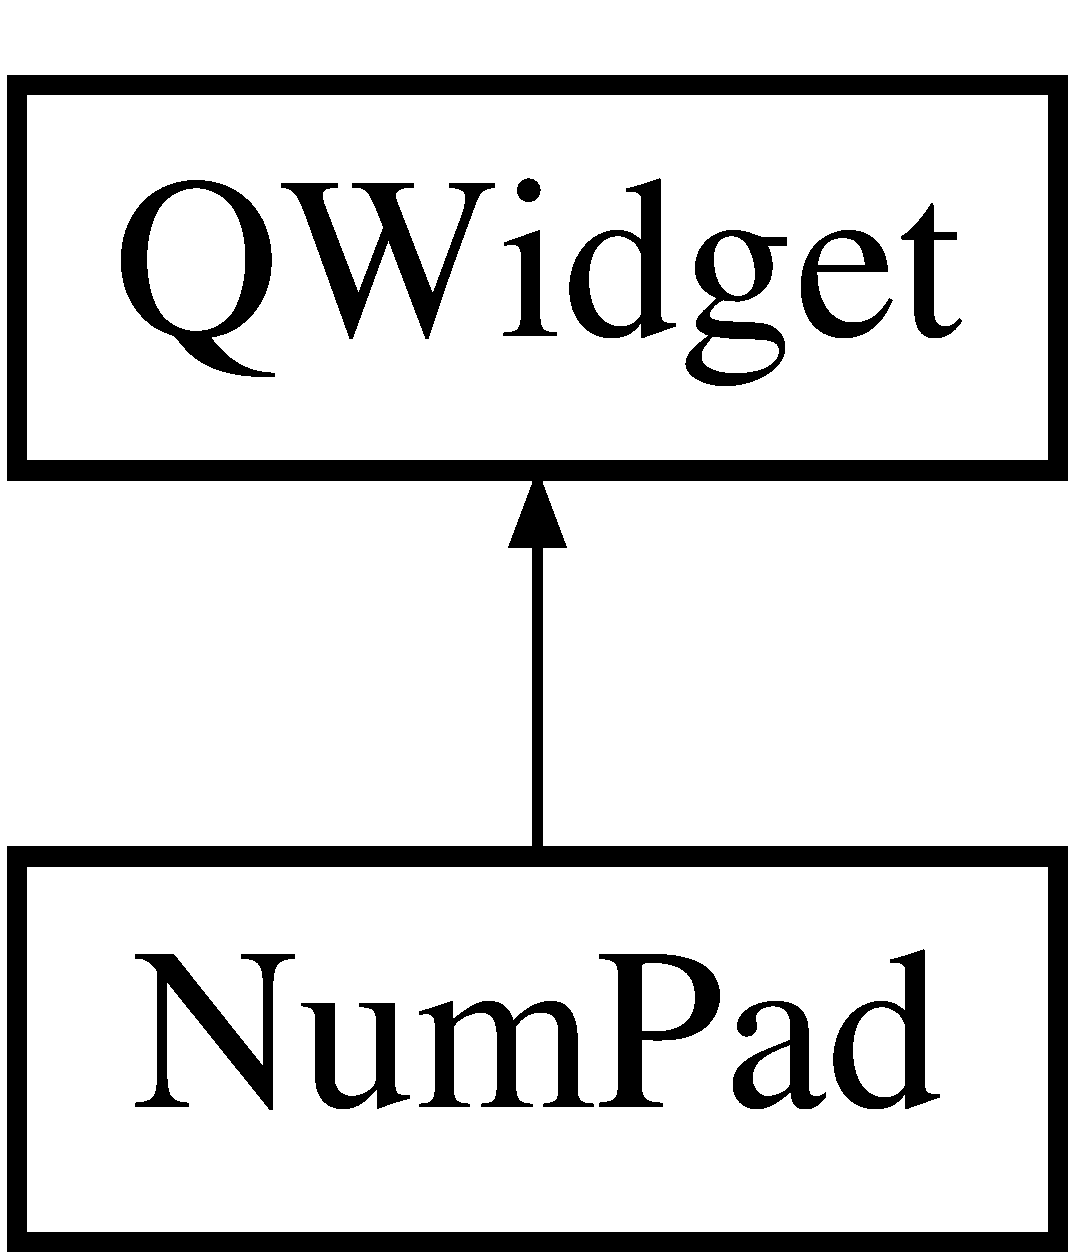
\includegraphics[height=2.000000cm]{class_num_pad}
\end{center}
\end{figure}
\subsection*{Public Slots}
\begin{DoxyCompactItemize}
\item 
\hypertarget{class_num_pad_ac6620373f360b666b71108b13946013a}{}\label{class_num_pad_ac6620373f360b666b71108b13946013a} 
void {\bfseries on\+Button\+Zero\+Clicked} ()
\item 
\hypertarget{class_num_pad_a6623d11d0e41f47e476f5e99a0d4eb71}{}\label{class_num_pad_a6623d11d0e41f47e476f5e99a0d4eb71} 
void {\bfseries on\+Button\+One\+Clicked} ()
\item 
\hypertarget{class_num_pad_a16eb90e6203c9d59eb0c6ea2697100c2}{}\label{class_num_pad_a16eb90e6203c9d59eb0c6ea2697100c2} 
void {\bfseries on\+Button\+Two\+Clicked} ()
\item 
\hypertarget{class_num_pad_a7e4ddab2ee993b84198b589b16305a76}{}\label{class_num_pad_a7e4ddab2ee993b84198b589b16305a76} 
void {\bfseries on\+Button\+Three\+Clicked} ()
\item 
\hypertarget{class_num_pad_afd185aa4de995f81384ca9d6c0f52af5}{}\label{class_num_pad_afd185aa4de995f81384ca9d6c0f52af5} 
void {\bfseries on\+Button\+Four\+Clicked} ()
\item 
\hypertarget{class_num_pad_aa494f765620859681fa7daac1b6dbc57}{}\label{class_num_pad_aa494f765620859681fa7daac1b6dbc57} 
void {\bfseries on\+Button\+Five\+Clicked} ()
\item 
\hypertarget{class_num_pad_a0eec28eb14ac08a0bd90eebcd43bfea6}{}\label{class_num_pad_a0eec28eb14ac08a0bd90eebcd43bfea6} 
void {\bfseries on\+Button\+Six\+Clicked} ()
\item 
\hypertarget{class_num_pad_a249c3837cc94eea7e2fdec57d78e1d6b}{}\label{class_num_pad_a249c3837cc94eea7e2fdec57d78e1d6b} 
void {\bfseries on\+Button\+Seven\+Clicked} ()
\item 
\hypertarget{class_num_pad_aefad78a1724a0962dc66df3f8b434a8a}{}\label{class_num_pad_aefad78a1724a0962dc66df3f8b434a8a} 
void {\bfseries on\+Button\+Eight\+Clicked} ()
\item 
\hypertarget{class_num_pad_a453339b8ce818824204f96607708c916}{}\label{class_num_pad_a453339b8ce818824204f96607708c916} 
void {\bfseries on\+Button\+Nine\+Clicked} ()
\item 
\hypertarget{class_num_pad_a153332f9a9b050037329d054d8cac6ae}{}\label{class_num_pad_a153332f9a9b050037329d054d8cac6ae} 
void {\bfseries on\+Button\+Dot\+Clicked} ()
\item 
\hypertarget{class_num_pad_abc4841a30a7777e207aebeb6020d9194}{}\label{class_num_pad_abc4841a30a7777e207aebeb6020d9194} 
void {\bfseries on\+Button\+Done\+Clicked} ()
\item 
\hypertarget{class_num_pad_a8e5af4566f4c3e5574a6867877ee795b}{}\label{class_num_pad_a8e5af4566f4c3e5574a6867877ee795b} 
void {\bfseries on\+Button\+Bksp\+Clicked} ()
\end{DoxyCompactItemize}
\subsection*{Public Member Functions}
\begin{DoxyCompactItemize}
\item 
\hypertarget{class_num_pad_ac35bfd6bb99a182c9073d80a09f3baf9}{}\label{class_num_pad_ac35bfd6bb99a182c9073d80a09f3baf9} 
{\bfseries Num\+Pad} (\hyperlink{class_client}{Client} $\ast$c)
\end{DoxyCompactItemize}
\subsection*{Public Attributes}
\begin{DoxyCompactItemize}
\item 
\hypertarget{class_num_pad_aeba02dbc3ca834bbd75f817855f5ecfb}{}\label{class_num_pad_aeba02dbc3ca834bbd75f817855f5ecfb} 
\hyperlink{class_client}{Client} $\ast$ {\bfseries client}
\end{DoxyCompactItemize}


The documentation for this class was generated from the following files\+:\begin{DoxyCompactItemize}
\item 
src/numpad.\+h\item 
src/numpad.\+cpp\end{DoxyCompactItemize}

\hypertarget{class_server}{}\section{Server Class Reference}
\label{class_server}\index{Server@{Server}}
Inheritance diagram for Server\+:\begin{figure}[H]
\begin{center}
\leavevmode
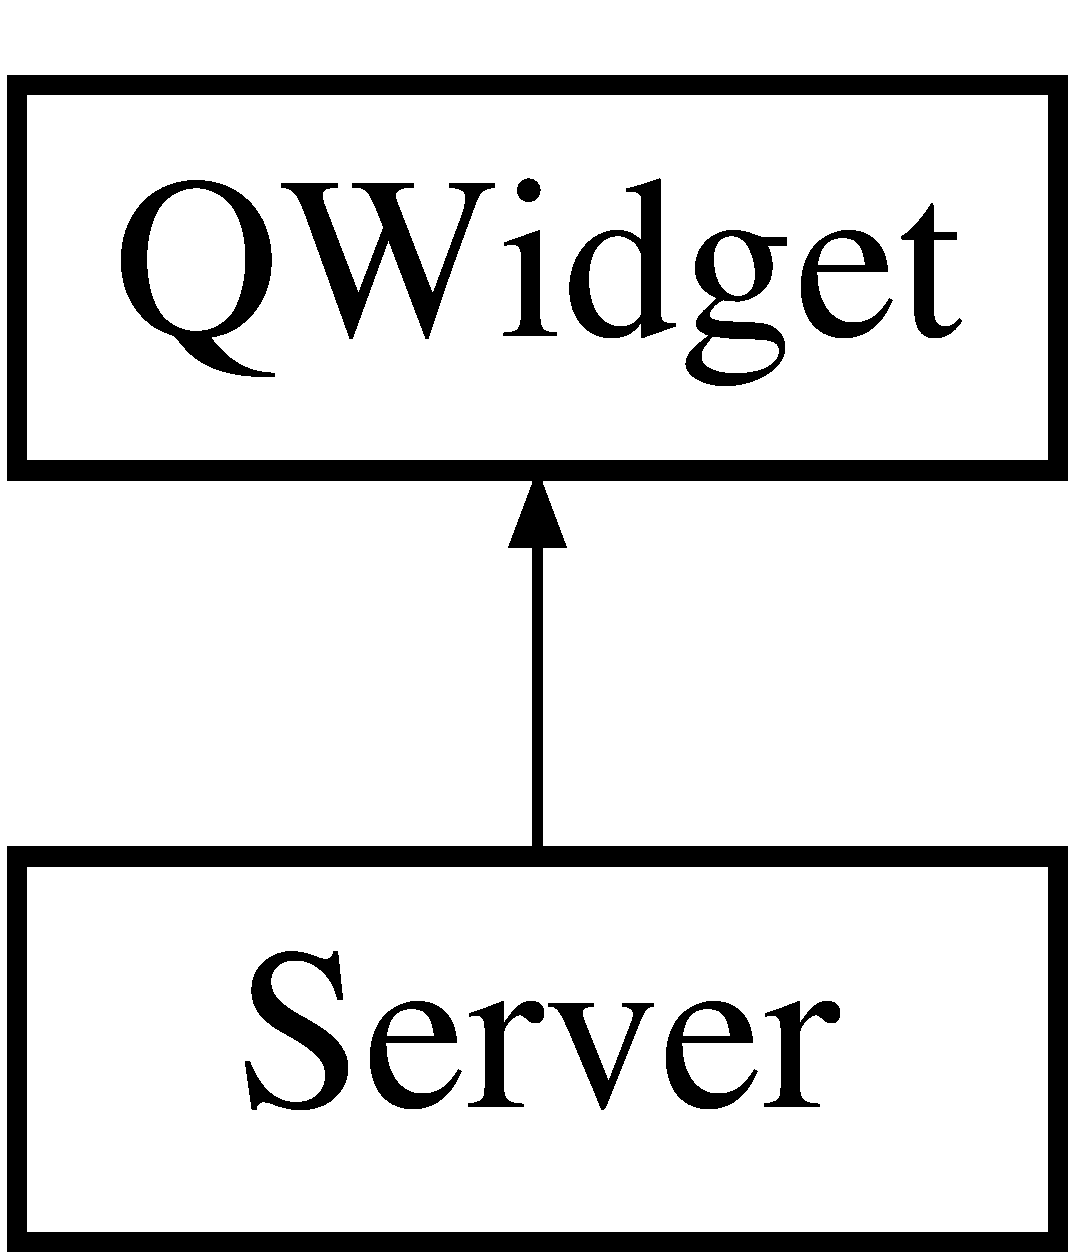
\includegraphics[height=2.000000cm]{class_server}
\end{center}
\end{figure}
\subsection*{Public Slots}
\begin{DoxyCompactItemize}
\item 
\hypertarget{class_server_a99f9b2f3521fb22772a61baf4f3c7bdc}{}\label{class_server_a99f9b2f3521fb22772a61baf4f3c7bdc} 
void {\bfseries on\+Exit\+Button\+Clicked} ()
\item 
\hypertarget{class_server_abe8ac23afc4d282f89ec9fac8e7bf7f3}{}\label{class_server_abe8ac23afc4d282f89ec9fac8e7bf7f3} 
void {\bfseries on\+Start\+Button\+Clicked} ()
\end{DoxyCompactItemize}
\subsection*{Public Member Functions}
\begin{DoxyCompactItemize}
\item 
\hypertarget{class_server_a0bf03b27b29ae4b969ec903f95041a17}{}\label{class_server_a0bf03b27b29ae4b969ec903f95041a17} 
{\bfseries Server} (Q\+Widget $\ast$parent=0)
\end{DoxyCompactItemize}


The documentation for this class was generated from the following files\+:\begin{DoxyCompactItemize}
\item 
src/server.\+h\item 
src/server.\+cpp\end{DoxyCompactItemize}

\hypertarget{class_traffic_light}{}\section{Traffic\+Light Klassenreferenz}
\label{class_traffic_light}\index{Traffic\+Light@{Traffic\+Light}}


Die Traffic\+Light-\/\+Klasse.  




{\ttfamily \#include $<$trafficlight.\+h$>$}

Klassendiagramm für Traffic\+Light\+:\begin{figure}[H]
\begin{center}
\leavevmode
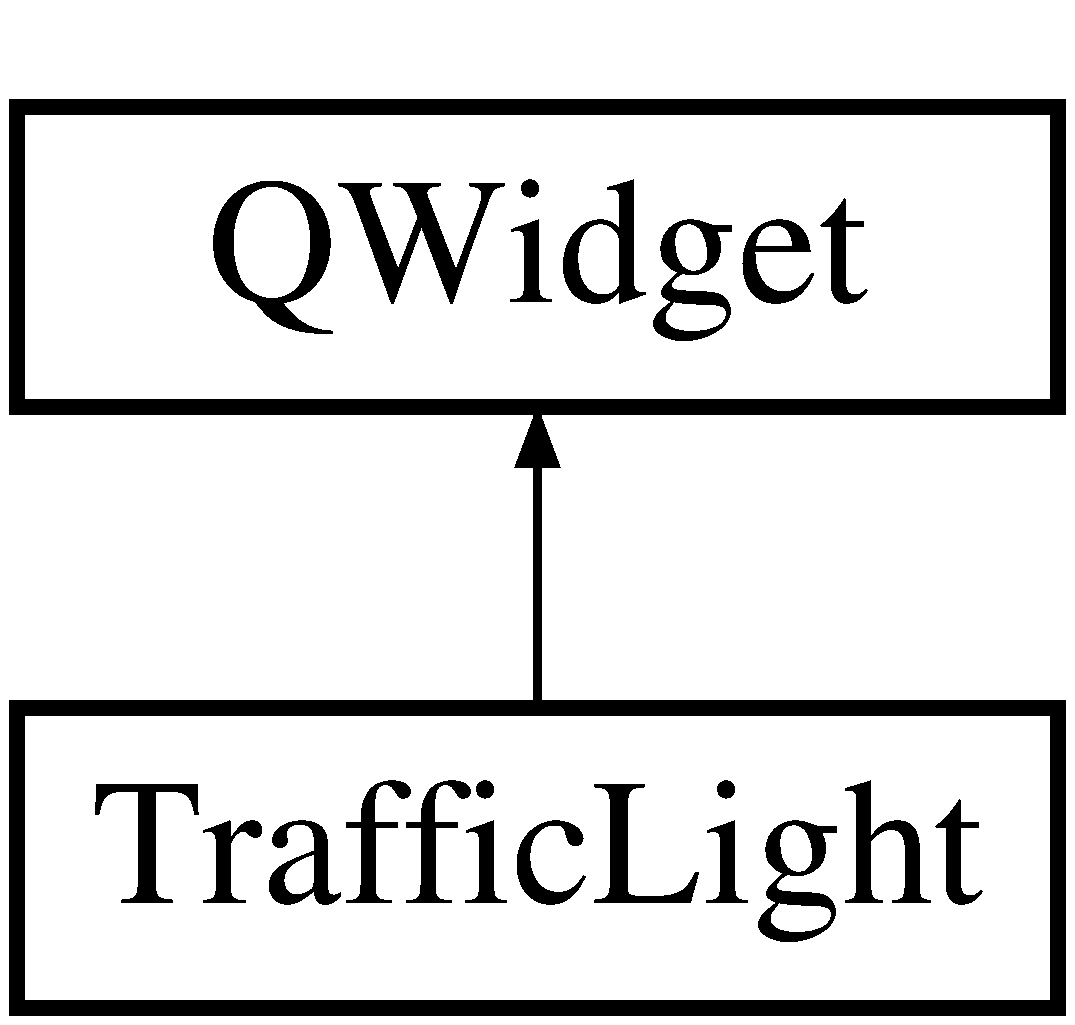
\includegraphics[height=2.000000cm]{class_traffic_light}
\end{center}
\end{figure}
\subsection*{Öffentliche Typen}
\begin{DoxyCompactItemize}
\item 
\hypertarget{class_traffic_light_a52ce5d9c3d0ec5aad2884db90fc10876}{}\label{class_traffic_light_a52ce5d9c3d0ec5aad2884db90fc10876} 
enum \hyperlink{class_traffic_light_a52ce5d9c3d0ec5aad2884db90fc10876}{color} \{ {\bfseries green}, 
{\bfseries red}, 
{\bfseries yellow}
 \}\begin{DoxyCompactList}\small\item\em Die drei Farben Grün, Rot, Gelb. \end{DoxyCompactList}
\end{DoxyCompactItemize}
\subsection*{Öffentliche Methoden}
\begin{DoxyCompactItemize}
\item 
\hyperlink{class_traffic_light_aa018a0285c92c087e48d3b16be3088ca}{Traffic\+Light} (Q\+Widget $\ast$parent=0)
\begin{DoxyCompactList}\small\item\em Der Traffic\+Light-\/\+Konstruktor. \end{DoxyCompactList}\item 
void \hyperlink{class_traffic_light_ad1e030e87446be2c976f5aedb4f511d5}{set\+Color} (\hyperlink{class_traffic_light_a52ce5d9c3d0ec5aad2884db90fc10876}{color} c)
\begin{DoxyCompactList}\small\item\em Setzt die Farbe. \end{DoxyCompactList}\end{DoxyCompactItemize}


\subsection{Ausführliche Beschreibung}
Die Traffic\+Light-\/\+Klasse. 

\subsection{Beschreibung der Konstruktoren und Destruktoren}
\hypertarget{class_traffic_light_aa018a0285c92c087e48d3b16be3088ca}{}\label{class_traffic_light_aa018a0285c92c087e48d3b16be3088ca} 
\index{Traffic\+Light@{Traffic\+Light}!Traffic\+Light@{Traffic\+Light}}
\index{Traffic\+Light@{Traffic\+Light}!Traffic\+Light@{Traffic\+Light}}
\subsubsection{\texorpdfstring{Traffic\+Light()}{TrafficLight()}}
{\footnotesize\ttfamily Traffic\+Light\+::\+Traffic\+Light (\begin{DoxyParamCaption}\item[{Q\+Widget $\ast$}]{parent = {\ttfamily 0} }\end{DoxyParamCaption})\hspace{0.3cm}{\ttfamily [explicit]}}



Der Traffic\+Light-\/\+Konstruktor. 


\begin{DoxyParams}{Parameter}
{\em parent} & \\
\hline
\end{DoxyParams}


\subsection{Dokumentation der Elementfunktionen}
\hypertarget{class_traffic_light_ad1e030e87446be2c976f5aedb4f511d5}{}\label{class_traffic_light_ad1e030e87446be2c976f5aedb4f511d5} 
\index{Traffic\+Light@{Traffic\+Light}!set\+Color@{set\+Color}}
\index{set\+Color@{set\+Color}!Traffic\+Light@{Traffic\+Light}}
\subsubsection{\texorpdfstring{set\+Color()}{setColor()}}
{\footnotesize\ttfamily void Traffic\+Light\+::set\+Color (\begin{DoxyParamCaption}\item[{\hyperlink{class_traffic_light_a52ce5d9c3d0ec5aad2884db90fc10876}{Traffic\+Light\+::color}}]{c }\end{DoxyParamCaption})}



Setzt die Farbe. 


\begin{DoxyParams}{Parameter}
{\em c} & \\
\hline
\end{DoxyParams}


Die Dokumentation für diese Klasse wurde erzeugt aufgrund der Dateien\+:\begin{DoxyCompactItemize}
\item 
src/\hyperlink{trafficlight_8h}{trafficlight.\+h}\item 
src/trafficlight.\+cpp\end{DoxyCompactItemize}

\hypertarget{class_welcome_screen}{}\section{Welcome\+Screen Class Reference}
\label{class_welcome_screen}\index{Welcome\+Screen@{Welcome\+Screen}}
Inheritance diagram for Welcome\+Screen\+:\begin{figure}[H]
\begin{center}
\leavevmode
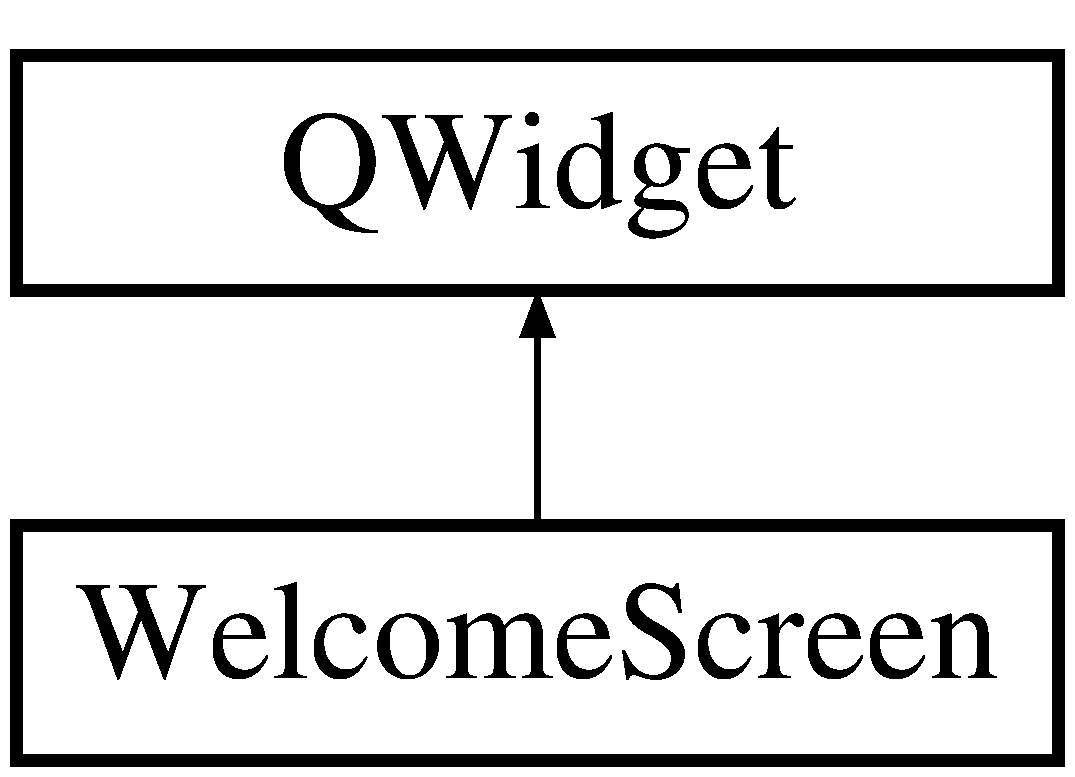
\includegraphics[height=2.000000cm]{class_welcome_screen}
\end{center}
\end{figure}
\subsection*{Public Slots}
\begin{DoxyCompactItemize}
\item 
\hypertarget{class_welcome_screen_adccaa9a1534c67f1fcd43245ff689b9e}{}\label{class_welcome_screen_adccaa9a1534c67f1fcd43245ff689b9e} 
void {\bfseries on\+Client\+Button\+Clicked} ()
\item 
\hypertarget{class_welcome_screen_ad4561643cb7feb6ad60e1daa097653d8}{}\label{class_welcome_screen_ad4561643cb7feb6ad60e1daa097653d8} 
void {\bfseries on\+Server\+Button\+Clicked} ()
\item 
\hypertarget{class_welcome_screen_a587ba35bfff39970d795906f253a52f8}{}\label{class_welcome_screen_a587ba35bfff39970d795906f253a52f8} 
void {\bfseries on\+Exit\+Button\+Clicked} ()
\end{DoxyCompactItemize}
\subsection*{Public Member Functions}
\begin{DoxyCompactItemize}
\item 
\hypertarget{class_welcome_screen_a5935d49d3bc2f3aae45db144bbbd4db2}{}\label{class_welcome_screen_a5935d49d3bc2f3aae45db144bbbd4db2} 
{\bfseries Welcome\+Screen} (Q\+Widget $\ast$parent=0)
\end{DoxyCompactItemize}


The documentation for this class was generated from the following files\+:\begin{DoxyCompactItemize}
\item 
src/welcomescreen.\+h\item 
src/welcomescreen.\+cpp\end{DoxyCompactItemize}

\chapter{File Documentation}
\hypertarget{client_8h}{}\section{src/client.h File Reference}
\label{client_8h}\index{src/client.\+h@{src/client.\+h}}


A brief description about this header file.  


{\ttfamily \#include $<$Q\+Widget$>$}\newline
\subsection*{Classes}
\begin{DoxyCompactItemize}
\item 
class \hyperlink{class_client}{Client}
\begin{DoxyCompactList}\small\item\em The \hyperlink{class_client}{Client} class. \end{DoxyCompactList}\end{DoxyCompactItemize}


\subsection{Detailed Description}
A brief description about this header file. 

A long description about this header file.

\begin{DoxyAuthor}{Author}
Andreas Hueber 

Thomas Breuss 
\end{DoxyAuthor}

\hypertarget{main_8cpp}{}\section{src/main.cpp-\/\+Dateireferenz}
\label{main_8cpp}\index{src/main.\+cpp@{src/main.\+cpp}}


Die main-\/\+Datei dieses Projekts.  


{\ttfamily \#include \char`\"{}welcomescreen.\+h\char`\"{}}\newline
{\ttfamily \#include $<$Q\+Application$>$}\newline
{\ttfamily \#include $<$Q\+File$>$}\newline
{\ttfamily \#include $<$Q\+Settings$>$}\newline
\subsection*{Funktionen}
\begin{DoxyCompactItemize}
\item 
int \hyperlink{main_8cpp_a0ddf1224851353fc92bfbff6f499fa97}{main} (int argc, char $\ast$argv\mbox{[}$\,$\mbox{]})
\begin{DoxyCompactList}\small\item\em Die main-\/\+Methode für das Projekt. \end{DoxyCompactList}\end{DoxyCompactItemize}


\subsection{Ausführliche Beschreibung}
Die main-\/\+Datei dieses Projekts. 

Das ist die Hauptdatei und Eingangsscript des Projekt \char`\"{}iperf G\+U\+I\char`\"{}.

\begin{DoxyAuthor}{Autor}
Andreas Hueber 

Thomas Breuss 

Tobias Merz 
\end{DoxyAuthor}


\subsection{Dokumentation der Funktionen}
\hypertarget{main_8cpp_a0ddf1224851353fc92bfbff6f499fa97}{}\label{main_8cpp_a0ddf1224851353fc92bfbff6f499fa97} 
\index{main.\+cpp@{main.\+cpp}!main@{main}}
\index{main@{main}!main.\+cpp@{main.\+cpp}}
\subsubsection{\texorpdfstring{main()}{main()}}
{\footnotesize\ttfamily int main (\begin{DoxyParamCaption}\item[{int}]{argc,  }\item[{char $\ast$}]{argv\mbox{[}$\,$\mbox{]} }\end{DoxyParamCaption})}



Die main-\/\+Methode für das Projekt. 


\begin{DoxyParams}{Parameter}
{\em argc} & Der Grösse des Argumente-\/\+Arrays \\
\hline
{\em argv} & Das Argumente-\/\+Array \\
\hline
\end{DoxyParams}
\begin{DoxyReturn}{Rückgabe}

\end{DoxyReturn}

%--- End generated contents ---

% Index
\backmatter
\newpage
\phantomsection
\clearemptydoublepage
\addcontentsline{toc}{chapter}{Index}
\printindex

\end{document}
